\documentclass[twocolumn]{article}
\usepackage[utf8]{inputenc}
\usepackage{ragged2e}
\usepackage{fancyhdr}
\usepackage{indentfirst}
\usepackage{graphicx}
\usepackage{caption}
\usepackage{amsmath}

\graphicspath{ {images/} }

\setlength\parindent{10pt}

\pagestyle{fancy}
\fancyhf{}
\rhead{J.Aubert, W.Detlor, J.Leung}
\lhead{An Elementary OCR System}
\cfoot{\thepage}

\begin{document}

\title{An Elementary Optical Character Recognition System}
\author{Jason Aubert, Will Detlor, Jesper Leung}
\date{December 2015}
\begin{titlepage}
\maketitle
\end{titlepage}



\maketitle

\begin{abstract}
\justify
This paper goes over an elementary implementation of a complete optical character recognition system, capable of recognizing handwritten digits from 0 to 9, and uppercase letters from A to Z. Prior to recognition, every image that is input into the system is thinned and scaled, with the option of processing multiple characters also available. Once scaled, each individual character is then put through the recognition system, which consists of the use of a statistical method where the ratio of black pixels to white pixels in certain zones of the image is calculated, and used to generate a feature vector to describe the input character. This feature vector is later compared to a large number of other feature vectors from test images in a database and the feature vector with the lowest Euclidean distance with the input image will then be used to recognize the character.
\end{abstract}

\section{Introduction}
An optical character recognition system, or OCR for short, is characterized by a conversion from images of handwritten or printed text into data that can be later used for processing by a computer system. OCR systems are typically used to process printed texts for applications such as digital storage, and electronic modifications. OCR systems can also be found in other applications, such as the translation of handwritten languages, as well as in text-to-speech implementations. \par
Through the use of various functions, this optical character recognition system is able to recognize images of handwritten digits from 0 to 9, as well as uppercase letters from A to Z. After processing, the system will then output the digit or letter that it believes to most closely represent the image that was inputted. This process is explored more in depth in the following section.  \par
This paper will then explore the results of the proposed method, through the use of 75 test images per digits to test the system’s accuracy, which will then be used to explore the limitations of the statistical method for feature extraction that is used in this OCR system. \par
Future considerations for improving the OCR system will then be explored in the penultimate section of this paper, where suggestions for future development are considered and discussed, and where areas of improvement within the current iteration of the system can be found. \par

\section{OCR System}
The OCR system we have written involves many steps to get from the initial character input to the character recognition output. The system was written in the python programming language and we implement the pillow library to assist with image handling.  The character is imported into the system as a grayscale image, we convert the image to a black and white.  The image is converted to black and white because the thinning algorithm used requires the image to be each white or black, and our feature vector calculates the amount of black pixels to the amount of white pixels.  After the character has been imported to the program correctly and converted to a black and white image, we check to see if there are multiple characters in the image[-------------------will------------------].  The program will then scale the image to a predetermine size so that all characters are the same size and this also helps with the speed of the program.  The image is padded with zeros after it has been scaled so that the thinning algorithm preforms correctly.  The thinning algorithm that we use is the ZS algorithm which was developed by T.Y. Zhang and C.Y. Suen.  After the image is scaled and thinned, we divide the image into sixteen zones.  Each zone will become an element in our feature vector array.  Each element in the array is calculated by counting the amount of black pixels in the zone and dividing that number by the total amount of pixels in that zone.  Once a value for each zone is found, the feature vector is compared to the database of test vectors.  For each character, 0 to 9 and A-Z in uppercase, we have four handwritten characters and one typed character. For the uppercase letters we used font Calibri and for the numbers we used font Arial.  We compare the characters feature vector to each vector in the database to determine which vector in the database has the closest Euclidean distance to the characters vector.  The one with the shortest Euclidean distance is determined to be a match and the value associated with that vector is output as the recognized character.  The user is shown the original image and the output character and is asked whether the system output the correct result. 
\section{Results}
The proposed recognition system was tested with 75 sample images for each number from 0 to 9, for a total of 750 test images (sample test in figure 3.1). These test images were compared against two separate sets of data within the database, one of which only contained numbers while the other data set contained both numbers from 0 to 9 and capital letters from A to Z in order to compare the effect on the recognition rate. Afterwards, five test images of each letter are tested against the numbers and letters data set. The results for each data set are examined below.

\begin{figure}[h]
\centering
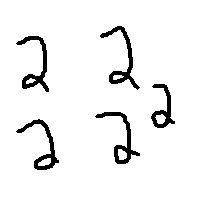
\includegraphics{2_10}
\caption*{Figure 3.1: Sample image tested with the proposed OCR system}
\end{figure}

\subsection{Numbers Only}
This data
\subsection{Numbers \& Letters}
\subsection{Letters}
\section{Extra features}
\subsection{Thinning}
Along with using the ZS algorithm in our program, we also started to implement the 20 rule algorithm developed by Maher Ahmed and Rabab Ward.  The 20 rule algorithm is an iterative algorithm, which at each iteration checks each pixel to see if the pixel is on the edge of the image, and if the pixel is on the edge then the pixel is deleted.  Once every pixel in the image has been checked, another iteration is ran until only a 1-pixel width skeleton of the image is left.  All 20 rules are implemented in the program correctly, but when the image has a width of two pixels then both pixels are deleted since both pixels are on an edge in the same iteration.  This happens because there was not enough time to fully implement the 20-rule algorithm correctly. With the 20-rule algorithm not working for images of 2 pixels in width, there are discontinuities in the input image which is why the program implements the ZS algorithm instead of the 20-rule algorithm.  If we used the 20-rule algorithm in the OCR system, the character recognition vector would have been off slightly which would affect our recognition rate.  The attempt to use the 20 thinning rules algorithm in the OCR system was to improve the 


\begin{figure}[h]
\centering
\includegraphics[scale=0.75]{20rulethin}
\caption*{Figure 4.1.1: Original image and the corresponding thinned image}
\end{figure}

\subsection{Filtering}
Although not a part of the recognition system, filtering is demonstrated in this OCR system as a proof of concept. To achieve this, the image is first padded to allow for the convolution operation to work fully. The convolution operation involves the use of a 3x3 matrix known as the “kernel”, which is used to modify the image pixel by pixel. The convolution operation takes each pixel in the target image and multiplies the surrounding pixels of the target image with those in the kernel, in order to form a sum that is then used to replace the target pixel in the image, as demonstrated in Figure 4.2. \par

\begin{figure}[h]
\centering
\begin{tabular}{ |c|c|c| } 
    \hline
    \(i_0\) & \(i_1\) & \(i_2\) \\
    \hline
    \(i_3\) & \(i_4\) & \(i_5\) \\ 
    \hline
    \(i_6\) & \(i_7\) & \(i_8\) \\ 
    \hline
\end{tabular}
\caption*{Figure 4.2.1: A 9x9 matrix representing the image}
\end{figure}

\begin{figure}[h]
\centering
\begin{tabular}{ |c|c|c| } 
    \hline
    \(k_0\) & \(k_1\) & \(k_2\) \\
    \hline
    \(k_3\) & \(k_4\) & \(k_5\) \\ 
    \hline
    \(k_6\) & \(k_7\) & \(k_8\) \\ 
    \hline
\end{tabular}
\caption*{Figure 4.2.2: A 9x9 matrix representing the kernel}
\label{Figure 4.2}
\end{figure}

\begin{figure}[h]
\centering
\begin{equation*}
i_4 = (k_0 * i_0) + (k_1 * i_1) + ... + (k_8 * i_8) 
\end{equation*}
\caption*{Figure 4.2.3: Convolution equation on pixel \(i_4\)}
\end{figure}

As can be seen above, a convolution operation on a single pixel involves the 8 surrounding pixels. As such, padding is necessary in order to properly apply convolution to edge pixels. While padding the image with pixel values of 0 will still allow for convolution of the entire image to work, padding the image with its edge values, while more complicated of an operation, nets a better result. This padding operation is seen below in Figure 4.2.4 \par

\section{Future Outlook}

\section{Conclusion}

\section{References}

\end{document}
